\chapter{Literature Review}
\label{ch:literature_review}
This work has conducted a literature review and existing tool exploration to 
identify problem that provide motivation for research. This chapter also presents a running example. The running example is used throughout this thesis to help introducing and explaining concepts, such as presenting related work (e.g. incrementality, state/change-based model persistence and comparison), explaining this work's proposed approaches to address the slow loading of change-based models, and discussing how change-based model persistence can be exploited to optimise model differencing and conflict detection.

\section{Running Example}
\label{sec:running_example_1}

\begin{figure}[ht]
  \centering
  \begin{subfigure}[t]{0.45\linewidth}
    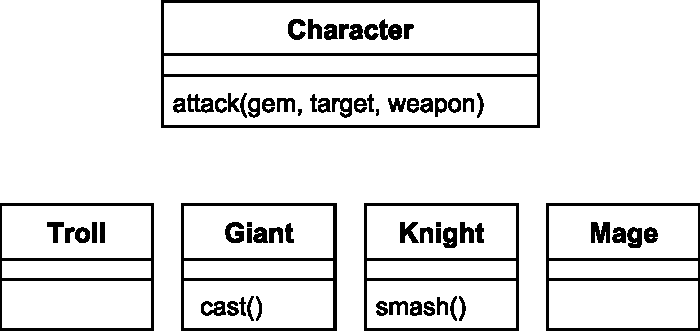
\includegraphics[width=\linewidth]{class_diagram_origin}
    \caption{original version (Jane's version)}
    \label{fig:class_diagram_origin}
  \end{subfigure}
  \\
  \begin{subfigure}[t]{0.45\linewidth}
    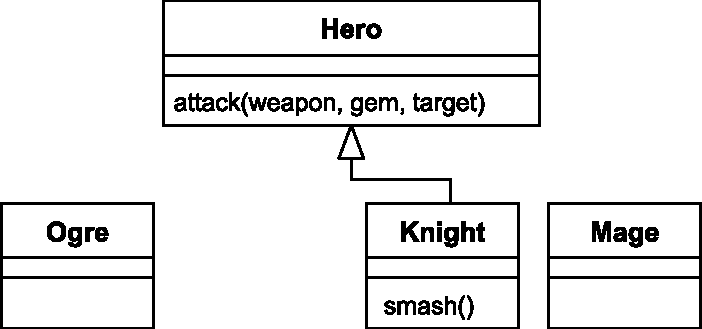
\includegraphics[width=\linewidth]{class_diagram_left}
    \caption{left version (Bob's version)}
    \label{fig:class_diagram_left}
  \end{subfigure}
  \hfill
  \begin{subfigure}[t]{0.45\linewidth}
    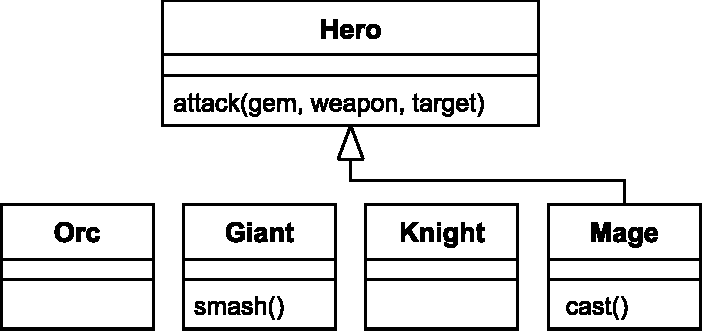
\includegraphics[width=\linewidth]{class_diagram_right}
    \caption{right version (Alice's version)}
    \label{fig:class_diagram_right}
  \end{subfigure}
  \caption{Three class diagrams of a Role Playing Game.}
  \label{fig:class_diagram_rpg}
\end{figure}

This chapter starts by introducing a running example. The example is used throughout this thesis to explain the solutions proposed in this research, such as loading optimisation of change-based models, hybrid model persistence, and change-based model differencing and conflict detection. The example is also used to explain how model differencing and conflict detection are performed in the related work, such as in EMF Compare \cite{emfcompare2018developer} and EMF Store \cite{emfstore2019what}. 

Let's say that there is a project to develop a simplified class diagram model of a Role Playing Game (RPG). Jane, as the technical leader, set up the initial model (Fig. \ref{fig:class_diagram_origin}). She then assigned this work to Bob and Alice. Both of them continued to work on the model and made some modification producing the models in Figures \ref{fig:class_diagram_left} and \ref{fig:class_diagram_right} respectively. Persisting these models in the standard XMI \cite{omg2018xmi} format produces three files as shown in Listings \ref{lst:xmimodel_origin}, \ref{lst:xmimodel_left}, and \ref{lst:xmimodel_right}.

\vspace{-20pt}
\begin{lstlisting}[style=xmi,caption={Simplified XMI file of the original version in Figure \ref{fig:class_diagram_origin}.},label=lst:xmimodel_origin]
<uml:Model>
  <packagedElement type=Class id="character" name="Character">
    <operation id="attack" name="attack">
      <parameter id="gem" name="gem"/>
      <parameter id="target" name="target"/>
      <parameter id="weapon" name="weapon"/>
    </operation>
  </packagedElement>
  <packagedElement type=Class id="troll" name="Troll"/>
  <packagedElement type=Class id="giant" name="Giant">
    <operation id="cast" name="cast"/>
  </packagedElement>
  <packagedElement type=Class id="knight" name="Knight">
    <operation id="smash" name="smash"/>
  </packagedElement>
  <packagedElement type=Class id="mage" name="Mage"/>
</uml:Model>
\end{lstlisting}

\vspace{-20pt}
\begin{lstlisting}[style=xmi,caption={Simplified XMI file of the left version in Figure \ref{fig:class_diagram_left}.},label=lst:xmimodel_left]
<uml:Model>
  <packagedElement type=Class id="character" name="Hero">
    <operation id="attack" name="attack">
      <parameter id="weapon" name="weapon"/>
      <parameter id="gem" name="gem"/>
      <parameter id="target" name="target"/>
    </operation>  
  </packagedElement>
  <packagedElement type=Class id="troll" name="Ogre"/>
  <packagedElement type=Class id="knight" name="Knight">
  <generalization id="leftGen" general="character"/>
    <operation id="smash" name="smash"/>
  </packagedElement>
  <packagedElement type=Class id="mage" name="Mage"/>
</uml:Model>
\end{lstlisting}

\vspace{-20pt}
\begin{lstlisting}[style=xmi,caption={Simplified XMI file of the right version of Figure \ref{fig:class_diagram_right}.},label=lst:xmimodel_right]
<uml:Model>
  <packagedElement type=Class id="character" name="Character">
    <operation id="attack" name="attack">
      <parameter id="gem" name="gem"/>
      <parameter id="weapon" name="weapon"/>
      <parameter id="target" name="target"/>
    </operation>
  </packagedElement>
  <packagedElement type=Class id="troll" name="Orc"/>
  <packagedElement type=Class id="giant" name="Giant">
    <operation id="smash" name="smash"/>
  </packagedElement>
  <packagedElement type=Class id="knight" name="Knight"/>
  <packagedElement type=Class id="mage" name="Mage">
    <generalization id="rightGen" general="character"/>
    <operation id="cast" name="cast"/>
  </packagedElement>
</uml:Model>
\end{lstlisting}

The company where Jane, Bob, and Alice work applies incremental model management in their development process. Applying incrementality allows them to manage their models automatically based on every change made to their models. For example, validating names of classes against a naming convention or to updating a class' documentation when the class is modified. Implementing such incrementality also comes with challenges (e.g., performance and cost for identifying changes; discussed in Section \ref{sec:the_key_challenge_of_incrementality}), and one solution that the company comes up with is, instead of only persisting the snapshots of models, they also persist the complete history of changes made to models in the form of change-based model persistence. 

\begin{lstlisting}[style=eol,caption={Change-based representation of the original version in Figure \ref{fig:class_diagram_origin}.},label=lst:cbp_origin]
session "Jane-01"
create character type Class
set character.name from null to "Character" 
create attack type Operation
set attack.name from null to "attack" 
add attack to character.operations at 0
create gem type Parameter
set gem.name from null to "gem" 
add gem to attack.parameters at 0
create target type Parameter
set target.name from null to "target" 
add target to attack.parameters at 1
create weapon type Parameter
set weapon.name from null to "weapon" 
add weapon to attack.parameters at 2
create troll type Class
set troll.name from null to "Troll" 
create giant type class
set giant.name from null to "Giant"
create cast type Operation
set cast.name from null to "smash"
add cast to giant.operations at 0
create knight type Class
set knight.name from null to "Knight"
create smash type Operation
set smash.name from null to "smash"
add smash to knight.operations at 0
create mage type Class
set mage.name from null to "Mage" 
\end{lstlisting}


For example, the complete history of changes made by Jane to construct the original version in Figure \ref{fig:class_diagram_origin} is also persisted in a change-based model representation as in Listing \ref{lst:cbp_origin}. The change events (Listing \ref{lst:cbp_left}) made by Bob is appended to Jane's original change events. Thus, the change events that represent Bob's version (Figure \ref{fig:class_diagram_left}) consists of the original change events and the change events (Listing \ref{lst:cbp_left}) made by him; only the appended changes are presented on the list. The change events that represents Alice's version (Figure \ref{fig:class_diagram_right}) is presented in Listing \ref{lst:cbp_right}. One clear advantage of change-based model persistence is that, from Listing \ref{lst:cbp_left}, we can immediately know all the changes made my Bob and Alice (starting from line 30) and identify all the elements that have been modified since Jane's version.  


\begin{lstlisting}[firstnumber=30,style=eol,escapechar=|,caption={The appended events made by Bob to produce the left version in Fig. \ref{fig:class_diagram_left} (left version).},label=lst:cbp_left]
session "Bob-01"|\label{line:cbp_left_30}|
create leftGen type Generalization|\label{line:cbp_left_31}|
set leftGen.general to character|\label{line:cbp_left_32}|
set troll.generalization to leftGen|\label{line:cbp_left_33}|
set character.name from "Character" to "Hero"|\label{line:cbp_left_34}|
unset troll.generalization from leftGen to null composite l1|\label{line:cbp_left_35}|
set knight.generalization to leftGen composite l1|\label{line:cbp_left_36}|
move target in attack.parameters from 1 to 2|\label{line:cbp_left_37}|
unset cast.name from "cast" to null composite l2|\label{line:cbp_left_38}|
remove cast from giant.operations at 0 composite l2|\label{line:cbp_left_39}|
delete cast composite l2|\label{line:cbp_left_40}|
unset giant.name from "Giant" to null composite l2|\label{line:cbp_left_41}|
delete giant composite l2|\label{line:cbp_left_42}|
set troll.name from "Troll" to "Ogre"|\label{line:cbp_left_43}|
\end{lstlisting}

\begin{lstlisting}[firstnumber=30,style=eol,escapechar=|,caption={The appended events made by Alice to produce the right version in Fig. \ref{fig:class_diagram_right} (right version).},label=lst:cbp_right]
session "Alice-01"|\label{line:cbp_right_30}|
move target in attack.parameters from 1 to 0|\label{line:cbp_right_31}|
remove smash from knight.operations at 0 composite r1|\label{line:cbp_right_32}|
add smash to giant.operations at 0 composite r1|\label{line:cbp_right_33}|
remove cast from giant.operations at 1 composite r2|\label{line:cbp_right_34}|
add cast to mage.operations at 0 composite r2|\label{line:cbp_right_35}|
create rightGen type Generalization|\label{line:cbp_right_36}|
set rightGen.general to character|\label{line:cbp_right_37}|
set troll.generalization to rightGen|\label{line:cbp_right_38}|
set character.name from "Character" to "Hero"|\label{line:cbp_right_39}|
unset troll.generalization from rightGen to null composite r3|\label{line:cbp_right_40}|
set mage.generalization to rightGen composite r3|\label{line:cbp_right_41}|
set troll.name from "Troll" to "Orc"|\label{line:cbp_right_42}|
\end{lstlisting}

 Let's say the complete scenario that produces the models in Figures \ref{fig:class_diagram_origin}, \ref{fig:class_diagram_left}, and \ref{fig:class_diagram_right} as wells Listings \ref{lst:cbp_origin}, \ref{lst:cbp_left}, and \ref{lst:cbp_right} occured according to the following story.

Jane, as the technical leader, set up the initial model. The records of events during setting up the initial is recorded in the CBMP in List. \ref{lst:cbp_origin}. She created a class \textsf{Character} that contains an operation \textsf{attack} with three parameters: \textsf{gem}, \textsf{target}, and \textsf{weapon} (lines 2-15). She also created four other classes; \textsf{Troll} (lines 16-17), \textsf{Giant} (lines 18-22), \textsf{Knight} (lines 23-27), and \textsf{Mage} (lines 28-29). She then pushed her work to a change-based version control system. If her work is visualised in state-based format, the model looks like in Fig. \ref{fig:class_diagram_origin}.

She then assigned this work to Bob and Alice. Both of them checked out this project to their own machine. Alice then started to continue the model. She then moved parameter \textsf{target} to the first place in operation \textsf{attack}'s parameters, because she thought it was more intuitive for programmers to think about the \textsf{target} first than the rest parameters (List. \ref{lst:cbp_right}, line 31). She also moved operation \textsf{smash} from class \textsf{Knight} to class \textsf{Giant} and operation \textsf{cast} from class \textsf{Giant} to class \textsf{Mage} as they are more reasonable to belong to their new classes (lines 32-35). Alice also created a generalisation relationship with id \textsf{rightGen} from class \textsf{Troll} to class \textsf{Character} (36-39). Bob also did the same thing except that his generalisation came with id \textsf{leftGen} (List. \ref{lst:cbp_left}, line 31-33). 

Later on, Jane then informed them that she wanted all good characters should be derived from a general, hero-like class, and the enemy should be the Orcs not Trolls. She also instructed that Bob should focus on developing class \textsf{Knight} and Alice on class \textsf{Mage}. In consequence, Alice then changed the name of class \textsf{Character} from ``Character'' to ``Hero'' (the id of class \textsf{Hero} is still \textsf{character}) (line 39). Again, Bob did the same thing. He also changed the name of class \textsf{Character} from ``Character'' to ``Hero'' (line 34). Instead of creating a new generalisation relationship, both of them preferred to move the generalisation relationships that they had created to their assigned classes. Alice moved generalisation \textsf{rightGen} from class \textsf{Troll} to class \textsf{Mage} (lines 40-41), and Bob move generalisation \textsf{leftGen} from class \textsf{Troll} to class \textsf{Knight} (lines 35-36). Bob also moved parameter \textsf{target} in operation \textsf{attack} to the last index as he thought setting target as the last parameter was intuitive (line 37), and deleted the class {Giant}, and unfortunately, he deleted class \text{Giant} accidentally (lines 38-42). The class diagrams of Bob and Alice's models are visualised in Figures \ref{fig:class_diagram_left} and \ref{fig:class_diagram_right} respectively. Lastly, Alice changed the \textsf{name} of class \textsf{Troll} to ``Orc'' (line 42) while Bob changed it to ``Ogre'' (line 43).  

In Listings \ref{lst:cbp_right} and \ref{lst:cbp_left}, we also introduce composite events -- lines with keyword \textsf{composite} -- that represent composite change events. 
Composite change events are events that should be treated as one composition -- identified with the same composite id. 
For example, moving an element from a container to another container is composite event since it consists of two change events: 
removing/unsetting the element from its source container and adding/setting it to its target container (lines 40-41 Listing \ref{lst:cbp_right}). 

\section{The Challenge of Incrementality}
\label{sec:the_key_challenge_of_incrementality}
To illustrate the key-challenge of incrementality, I use the example in Fig. \ref{fig:class_diagram_rpg}. Let's say that after every modification to the model in Fig. \ref{fig:class_diagram_origin}, the model needs to be:

\begin{itemize}
  \item Validated against a naming convention that the name of a class should start with an uppercase.
  \item Transformed into a number of documentation files through a model-to-text transformation. Each class should have a documentation file.
\end{itemize}

Models in Figures \ref{fig:class_diagram_origin} and \ref{fig:class_diagram_left} are two consecutive versions. When the validation constraint is evaluated against the first version of the model (Fig. \ref{fig:class_diagram_origin}), it verifies that all the classes' names starts with a uppercase, and the model-to-text transformation then produces four documentation files that correspond to the classes in the model. In the sequel, in Fig. \ref{fig:class_diagram_left}, the model is updated by Bob. He applies several changes, such as renaming class \textsf{Character} to \textsf{Hero} and class \textsf{Troll} to \textsf{Ogre} and deleting class \textsf{Giant}.

A non-incremental model validation engine would treat the model of 
Fig. \ref{fig:class_diagram_left} as if it was a new model and would evaluate 
the constraint above against every class in the model. 
An incremental model validation engine, on the other hand, would identify 
that the previously established satisfaction of the constraint for classes 
\textsf{Knight} and \textsf{Mage} cannot have been possibly compromised by the changes made, and would only re-evaluate the constraint for classes \textsf{Character} and \textsf{Troll} (class \textsf{Giant} is deleted so it is not evaluated). 

Similarly, a non-incremental model-to-text transformation would generate 
and overwrite all documentation files. On the contrary, an 
incremental model-to-text transformation, would identify that it only needs to delete the documentation file of class \textsf{Giant} and generate documentation files for classes \textsf{Character} and \textsf{Troll} -- but not the documentation files of classes \textsf{Knight} and \textsf{Mage}, as these cannot have been affected by the changes made to the model.

While the overhead of executing transformations and validation constraints 
on small models like the one in Fig. \ref{fig:class_diagram_origin} is negligible, non-incremental execution can become a significant bottleneck for large evolving models. As stressed in Selic's seminal work \cite{selic2003pragmatics}, with reference to model-to-text transformation, ``... \textsf{this is particularly true in the latter phases of the development cycle when programmers make many small changes as they fine-tune the system. To keep this overhead low, it is crucial for the code generators to have sophisticated change impact analysis capabilities that minimize the amount of code regeneration}''.

As demonstrated by the pioneering work of Egyed \cite{egyed2011automatically}, 
to achieve incremental re-execution of (deterministic) queries on 
structured models, an execution engine needs to:

\begin{enumerate}
  \item Record model element property accesses during the initial execution of the queries;
  \item Identify new and deleted elements and modified model element properties in the new version of the model;
  \item Combine the information collected in the steps above to identify the subset of (potentially) affected rules/queries/templates that need to be re-executed.
\end{enumerate}

To illustrate this, this example uses an OCL implementation of the domain-specific constraint in List. \ref{lst:constraint}.

\begin{lstlisting}[style=ocl,caption={OCL constraint requiring that a class should start with an uppercase.},label=lst:constraint]
context Class
inv UpperCase: self.name->subtring(1,1) == self.name->subtring(1,1)->toUpper()
\end{lstlisting}

\begin{table}[ht]
  \centering
  \caption{Property-access trace of the evaluation of the constraint in List. \ref{lst:constraint} on the model of Fig. \ref{fig:class_diagram_origin}.}
  \begin{small}
  \begin{tabular}{p{4cm} p{2.1cm} p{2cm} p{2.1cm}}
    \hline 
    \textbf{Constraint} & \textbf{Context} & \textbf{Accessed Element} & \textbf{Accessed Property} \\ 
    \hline 
    \textsf{Class.UpperCase}  & \textsf{character} & \textsf{character} & \textsf{name} \\ 
    \textsf{Class.UpperCase}  & \textsf{troll} & \textsf{troll} & \textsf{name} \\ 
    \textsf{Class.UpperCase}  & \textsf{giant} & \textsf{giant} & \textsf{name} \\ 
    \textsf{Class.UpperCase}  & \textsf{knight} & \textsf{knight} & \textsf{name} \\
    \textsf{Class.UpperCase}  & \textsf{mage} & \textsf{mage} & \textsf{name} \\
    \hline 
  \end{tabular} 
  \end{small}
  \label{tab:property_access_trace}
\end{table}

During the initial evaluation of the constraint on the model of Fig. \ref{fig:class_diagram_origin}, an incremental OCL engine would compute the property access trace displayed in Table \ref{tab:property_access_trace} as a side-product. Now, when the model is updated (Fig. \ref{fig:class_diagram_left}), the execution engine can identify that:

\begin{itemize}
  \item There is an element deleted in the model (class \textsf{Giant}) for which the constraint is not necessary to be evaluated;
  \item The value of property \textsf{name} of classes \textsf{Character} and \textsf{Troll} have changed, and as such, the constrain needs to be re-evaluated on this elements.
\end{itemize}

Egyed has shown that the property-access recording approach is applicable to queries of arbitrary complexity, 
as long as they are deterministic. More recent work has shown that variants of this approach can be used to 
achieve incrementality in a wide range of model processing operations, including model-to-model 
transformation \cite{jouault2010towards}, model-to-text transformation \cite{DBLP:conf/ecmdafa/OgunyomiRK15}, 
model validation, and pattern matching \cite{DBLP:conf/ecmdafa/RathHV12}---as long as changes to models can be 
precisely identified (step 2 in the list above).

\section{Identifying Changes in Models}
\label{sec:identifying_changes_in models}
There are two approaches in the literature for identifying changes in models 
in order to enable incremental re-execution of model processing operations.

\textbf{Notifications}. In this approach, the incremental execution 
engine needs to hook into the notification facilities 
provided by the modelling tool through which the developer edits the model, 
so that the engine can directly receive notifications as soon as 
changes happen (e.g. class \textsf{giant} has been deleted, class \textsf{character} has been renamed to ``Hero''). 
This is an approach taken by the IncQuery incremental pattern matching 
framework \cite{DBLP:conf/ecmdafa/RathHV12} and the ReactiveATL incremental model-to-model 
transformation engine \cite{DBLP:conf/ecmdafa/OgunyomiRK15}. The main advantage of this 
approach is that precise and fine-grained change notifications are provided 
for free by the modelling tool (and thus do not need to be computed by the 
execution engine---which as discussed below can be expensive and inefficient). 
On the downside, this approach is a poor fit for collaborative development 
settings where modelling and automated model processing activities are 
performed by different members of the team.

\textbf{Model Differencing}. This approach eliminates the coupling between 
modelling tools and incremental execution engines. Instead of depending on 
live notifications, in this approach the developer in charge of automated model 
processing, needs to have access to a copy of the last version of the model that the model processing program (e.g. the model-to-text transformation) was 
executed upon, so that it can be compared against the current version of 
the model (e.g. using a model-differencing framework such as SiDiff or 
EMFCompare) and the delta can be computed on demand. The main advantage of 
this approach is that it works well in a collaborative development environment 
where typically developers have distinct roles and responsibilities. On the 
downside, model comparison and differencing are computationally expensive and 
memory-greedy (both versions of the model need to be loaded into memory before 
they can be compared), thus largely undermining the time and resource saving 
potentials of incremental re-execution. 

In summary, incremental model processing currently delivers significant 
performance benefits only in a single-developer environment where the modeller 
is also responsible for performing all the (incremental) model processing 
operations. As a result, in collaborative development environments, 
developers need to either forgo incremental model processing altogether 
or to work around this limitation by manually steering model processing 
programs to process only subsets of their models, which is cumbersome and 
error prone.

\section{A Novel Solution to Incrementality}
\label{sec:a_novel_solution_to_incrementality}
A novel solution to incrementality should be able to deliver the advantages of both notification and model differencing approaches while eliminate their drawbacks. To realize such solution, this work comes with an idea that models can be persisted in their complete history of changes, a.k.a. change-based model persistence, as opposed to state-based model persistence that persists models in their snapshots at a time. In change-based model persistence, information about changes that have been applied to models can be preserved, and the persistence can be shared across the members of a team, for example through Version Control Systems (e.g., SVN, Git).The proposed change-based model persistence is discussed later in Chapter \ref{ch:change_based_model_persitence}. 

Moreover, change-based model persistence also can be exploited to optimise model comparison to only compares versions of a model on parts that have only been changed since their last shared common version. In other words, not every element of the versions is compared which can lead to a faster model comparison. This solution is discussed later in Chapters \ref{ch:model_differencing} and \ref{ch:conflict_detection}. 

\section{Change vs. State-based Persistence}
\label{sec:change_based_vs_state_based_persistence}
The concept of change-based persistence is not new and has been used in persisting changes of software, object-oriented databases, hierarchical documents, and models 
\cite{DBLP:journals/entcs/RobbesL07,DBLP:conf/sde/LippeO92,DBLP:conf/caise/IgnatN05,koegel2010emfstore}. 

The nature of change-based persistence give us two advantages. First, it contains finer-granularity information (e.g. types of changes, the order of the changes, elements that were changed, previous values, etc.) of changes which can improve the accuracy of change detection \cite{DBLP:journals/entcs/RobbesL07,DBLP:conf/sde/LippeO92,DBLP:conf/caise/IgnatN05,mens2002state}. Second, it records changes ordered manner which means that changes made to a model can be identified sequentially without having to explore and compare all elements of compared versions of models \cite{DBLP:conf/edoc/KoegelHLHD10}. The advantages to detect changes more precisely and much faster can then have positive knock-on effects on supporting (1) developers compare and merge models in collaborative modelling environments \cite{DBLP:conf/sde/LippeO92,DBLP:conf/caise/IgnatN05,koegel2010emfstore}, and (2) incremental model management \cite{jouault2010towards,DBLP:conf/ecmdafa/OgunyomiRK15, DBLP:conf/ecmdafa/RathHV12}. Moreover, changed-based persistence contains abundant information which can be exploited for analytics \cite{DBLP:journals/entcs/RobbesL07}.


Nevertheless, change-based persistence also comes with downsides, such as ever-growing model files 
\cite{DBLP:journals/entcs/RobbesL07,DBLP:conf/edoc/KoegelHLHD10} and increased model loading time \cite{mens2002state}
which increase storage and computation costs. A model that is frequently modified will increase considerably in file size 
since every change is added to the file. The increased file size (proportional to the number of persisted changes) will, 
in turn, increase the loading time of the model since all changes have to be replayed to reconstruct the model's 
eventual state. 

These downsides have to be mitigated to enable the practical adoption of change-based persistence. 
One approach to reducing the file size of change-based models is by removing changes that do not affect the eventual 
state of the model. For the increased loading time, it can be mitigated by ignoring -- i.e. not replaying -- changes 
that are cancelled out by later changes or employing change-based and state-based persistence side-by-side so that the
benefits of state-based persistence on loading time can be obtained. 

Other downsides are change-based persistence requires 
integration with existing tools -- since it is still a non-standard approach -- for its adoption \cite{koegel2010emfstore}, 
and still has limited support for standard, text-based version controls for collaborative development \cite{koegel2010emfstore}. 
These downsides can be addressed by developing a change-based persistence plugin for a specific development environment 
(e.g. Eclipse) and persisting changes in text-based format to support text-based version controls (e.g. Git, SVN).

%3-layer metamodelling architectures such as EMF and MOF. 
\begin{table}[t!]
    \centering
    \caption{The advantages and downsides between change-based and state-based persistence.}
    \label{table:advantages_drawbacks}
    \begin{tabular}
        {|>{\centering\arraybackslash}p{1.1cm}|>{\centering\arraybackslash}p{1.1cm}|>{\centering\arraybackslash}p{5cm}|>{\centering\arraybackslash}p{5cm}|}
        \hline 
        \multicolumn{2}{|c|}{\textbf{Dimensions}}&\textbf{Change-based Approach}&\textbf{State-based Approach}\\
        \hline 
        \multicolumn{2}{|p{2.2cm}|}{\centering Advantages} &
        \begin{minipage}[t]{5cm}
            \raggedright
            \begin{itemize}[leftmargin=9pt]
                \setlength\itemsep{2pt}
                \item[-] Faster for detecting changes \cite{DBLP:conf/edoc/KoegelHLHD10}
                \item[-] More accurate, carry semantic information \cite{DBLP:journals/entcs/RobbesL07,DBLP:conf/sde/LippeO92,DBLP:conf/caise/IgnatN05,mens2002state}  
                \item[-] Faster and more accurate for comparison and merging \cite{DBLP:conf/sde/LippeO92,DBLP:conf/caise/IgnatN05,koegel2010emfstore}
                \item[-] Information carried is useful for analytics \cite{DBLP:journals/entcs/RobbesL07}
            \end{itemize}
        \end{minipage}
        & 
        \begin{minipage}[t]{5cm}
            \raggedright
            \begin{itemize}[leftmargin=9pt]
                \setlength\itemsep{2pt}
                \item[-] Faster for loading large models \cite{DBLP:conf/models/Espinazo-PaganCM11,daniel2016neoemf,eclipse2019cdo}
                \item[-] A default standard, no need integration with existing tools \cite{koegel2010emfstore}  
            \end{itemize}
        \end{minipage}
        \\
        \hline
        \multicolumn{2}{|p{2.2cm}|}{\centering Disadvantages} & \begin{minipage}[t]{5cm}
            \raggedright
            \begin{itemize}[leftmargin=9pt]
                \setlength\itemsep{2pt}
                \item[-] Increased record size \cite{DBLP:journals/entcs/RobbesL07,DBLP:conf/edoc/KoegelHLHD10}
                \item[-] Is not efficient for replaying (loading) for long records \cite{mens2002state}
                \item[-] Limited supports for standard, text-based version controls (e.g. GitHub) \cite{koegel2010emfstore} 
                \item[-] Not a standard, need integration with existing tools \cite{koegel2010emfstore} 
            \end{itemize}
        \end{minipage}
        & 
        \begin{minipage}[t]{5cm}
            \raggedright
            \begin{itemize}[leftmargin=9pt]
                \setlength\itemsep{2pt}
                \item[-] Slower for saving changes  \cite{mens2002state,daniel2016neoemf,DBLP:conf/models/Espinazo-PaganCM11}
                \item[-] Slower for comparison \cite{DBLP:conf/edoc/KoegelHLHD10}
                \item[-] Less accurate, does not carry semantic information \cite{mens2002state,DBLP:conf/edoc/KoegelHLHD10}  
            \end{itemize}
        \end{minipage}
        \\
        \hline
    \end{tabular} 
\end{table}

In contrast, state-based persistence has several advantages over change-based persistence. First, since it is the default standard of persisting models, most of the available modelling tools support this kind of persistence thus there is no need for integration with existing tools \cite{koegel2010emfstore}. Second, it is faster in loading models since there is no need to replay all changes as in change-based persistence. Also, applying lazy loading -- elements of models are not loaded upfront -- enable faster CRUD (create, read, update, delete) operations \cite{DBLP:conf/models/Espinazo-PaganCM11,daniel2016neoemf}. 

Compared to change-based persistence, state-based persistence has several downsides. First, it is slower than change-based persistence in saving changes \cite{mens2002state}. Even thought its backends already implemented lazy loading, it still needs to undergo certain indexing mechanism to persist changes \cite{daniel2016neoemf,DBLP:conf/models/Espinazo-PaganCM11,eclipse2019cdo}. Second, state-based persistence does not have any records of recent elements that have been changed in a model. Thus, every element has to be checked for differences which can be less efficient if the comparison is performed in change-based format \cite{DBLP:conf/edoc/KoegelHLHD10}. Third, since comparison in state-based format requires deriving differences through a diffing process -- not based on actual change records, it can be less accurate than comparison in change-based persistence which is provided with more information to detect changes accurately \cite{mens2002state,DBLP:conf/edoc/KoegelHLHD10}. The summary of 
the advantages and downsides between change-based and state-based persistence are presented in
Table \ref{table:advantages_drawbacks}.

\section{The State of Art of Model Persistence}
\label{sec:the_state_of_art_of_model_persistence}
By default, modelling tools that support the 3-layer metamodelling architectures of Eclipse Modelling Framework (EMF) \cite{steinberg2008emf} employ state-based persistence to persist models in Metadata Interchange (XMI) format. XMI is a standard issued by Object Management Group (OMG) for exchanging metadata information via Extensible Markup Language (XML) \cite{omg2018xmi}. 

There are several non-XMI approaches to state-based model persistence that use relational or NoSQL databases. For example, EMF Teneo \cite{eclipse2017teneo} persists EMF models in relational databases, while Morsa \cite{DBLP:conf/models/Espinazo-PaganCM11} persist models in documents with MongoDB backend \cite{mongodb}, and NeoEMF \cite{daniel2016neoemf} persists models in multi NoSQL backends (Graph, Map, Column). However, none of these approaches provides built-in support for versioning and models are eventually stored in binary files/folders which are known to be a poor fit for text-oriented version control systems like Git and SVN. Connected Data Objects (CDO) \cite{eclipse2019cdo}, which provides support for database-backed model persistence, also provides collaboration facilities, but CDO adoption necessitates the use of a separate version control system (e.g. a Git repository for code and a CDO repository for models), which introduces fragmentation and administration challenges \cite{barmpis2014evaluation}. Similar challenges arise in relation to other model-specific version control systems such as EMFStore \cite{koegel2010emfstore}.

\section{The State of Art of Model Comparison}
\label{sec:the_state_of_art_of_model_comparison}
The history of diffing can be tracked back to the presence of \textsf{diff} program on Unix or Unix-like platform \cite{hunt1976algorithm}. The program can perform diffing that is comparing text files ``in order to determine how or whether they differ'' \cite{diff}. Diffing basically is about finding the longest common subsequence between two or more sequences which commonly known as the Longest Common Subsequence (LCS) algorithms \cite{bergroth2000lcs}. This problem is equivalent to the Shortest Edit Script (SES) problem that is to find the smallest number of editing (add and delete) in order to make a sequence equal to another sequence \cite{DBLP:journals/algorithmica/Meyers86}. LCS or SES algorithms are commonly implemented by Version Control Systems, such as SVN \cite{svn-diff} and Git \cite{git-diff}, in their \textsf{diff} programs to identify differences between versions of files.   

Applying this diffing approach to some non-text artefacts, such as XML \cite{w3c-xml} and Ecore models \cite{steinberg2008emf}, is not straightforward since they have different characteristics to text files. For example, XML is a hierarchical document with a tree structure; one node can contains other nodes. The unique feature of XML is that its containment is  unordered whereas in text differencing order is a necessary feature. This has been addressed by Wang et al. \cite{wang2003xdiff} by exploiting key XML  structure characteristics. Diffing Ecore models is even more complex since the models support multiple characteristics of features, such as attribute/reference, literal/object values, single/multiple values, containment/non-containment, etc \cite{steinberg2008emf}. 

There are several existing tools for model differencing. Beyond EMF Compare \cite{emfcompare2018developer}, which this study used for comparative evaluation due to its maturity and ongoing development activity, tools such as SiDiff \cite{Treude2007SiDiff} and DSMDiff \cite{lin2009dsmdiff} also provide language-agnostic graph-based model comparison, with some room for configuration (e.g., assigning different weights to features of types in the language). Additional expressive power -- at the cost of increased complexity and configuration effort -- is offered by dedicated comparison languages such as the Epsilon Comparison Language, which can be used to compare both homogeneous and heterogeneous models \cite{kolovos2009ecl}. All of these tools works with state-based persistence to identify differences between models.

This work does not aware of any other work that targets comparison of change-based models persisted in text files. Only EMF Store \cite{koegel2010emfstore} identified addresses change-based model comparison but it persists models in its own dedicated backend system. Database-backed model persistence and version control solutions such as CDO \cite{eclipse2019cdo} and EMF Store provide diffing capabilities between different versions of the same model without requiring models to be fully loaded into memory, however they present integration challenges with mainstream software engineering tools (e.g., continuous integration systems, backup and restore facilities) which are typically file-based, and their performance can degrade as more models/users are added to a repository, since all models are effectively stored in a single database \cite{KolovosRMPGCLRV13}. 

\section{State-based Model Differencing}
\label{sec:state-based_model_differencing}
Referring to the example in Section \ref{sec:running_example_1}, at one time, Bob decides to compare his model to Alice's model because he is interested to analyse the differences between their models. Bob then uses a model differencing tool and perform state-based model differencing. 
In state-based model differencing, comparing models commonly consists of two steps: \emph{matching} and \emph{diffing}.
The matching process establishes matches between the elements of both models, to determine the elements in the left model that correspond to elements in the right model. Generally, the matching process iterates through all the elements of the models being compared and matches them by their identifiers or through a similarity mechanism  \cite{DBLP:conf/sfm/BroschKLSWW12,emfcompare2018developer}. The diffing process then identifies differences between the matched elements \cite{DBLP:conf/sfm/BroschKLSWW12,emfcompare2018developer}. 

In our example, the matching process in state-based comparison -- as performed by EMF Compare \cite{emfcompare2018developer} -- iterates through all the elements of both models and matches them using their identifiers. The matching process yields 10 matches: $m_1$ = (\textsf{character}, \textsf{character}), $m_2$ = (\textsf{attack}, \textsf{attack}), $m_3$ = (\textsf{gem}, \textsf{gem}), $m_4$ = (\textsf{weapon}, \textsf{weapon}), $m_5$ = (\textsf{target}, \textsf{target}), $m_6$ = (\textsf{troll}, \textsf{troll}), $m_7$ = (\textsf{knight}, \textsf{knight}), $m_8$ = (\textsf{smash}, \textsf{smash}), and $m_9$ = (\textsf{mage}, \textsf{mage}), and 3 unmatched elements, $um_1$ = (-, \textsf{giant}), $um_2$ = (-, \textsf{rightGen}), $m_3$ = (-, \textsf{cast}), and $um_4$ = (\textsf{leftGen}, -). 

The diffing process then iterates through all the matches and unmatched elements and uses an LCS algorithm to identify their differences. During iterating the matches, in the second match $m_2$, it identifies that, in order to make the left feature \textsf{parameters} equal to the right feature \textsf{parameters}, parameter \textsf{gem} has to be moved from index 1 to 0 (diff $ds_1$). It is important to note that the employed LCS algorithm does not detect the different position of parameter \textsf{weapon}; it only identifies the minimum number of differences which if all are resolved unidirectionally can make both models equal. Otherwise, the number becomes less optimal -- not minimum.

In the six match $m_6$, The diffing process identifies that the classes \textsf{troll} are different in their \textsf{name}. The left \textsf{troll}'s \textsf{name} is ``Ogre'' while the other \textsf{troll}'s \textsf{name} is ``Orc'' (diff $ds_2$). In the eight match $m_8$, the diffing process identifies that the containers of operation \textsf{smash} are different. Thus, element \textsf{smash} has to be move from \textsf{knight}'s \textsf{operations} to \textsf{giant}'s \textsf{operations} (diff $ds_3$). For the other matches, the diffing process does not identify any differences. 

From the unmatched elements ($um_1$, $um_2$, $um_3$, and $um_4$), the diffing process identifies that, in order to make the left model equal to the right model, class \textsf{giant} has to be added to the left model's resource at index 2 (diff $ds_4$), generalization \textsf{rightGen} has to be added to class \textsf{mage}' s \textsf{generalization} (diff $ds_5$), operation \textsf{cast} has to be added to class \textsf{mage}'s \textsf{operations} (diff $ds_6$), and  generalization \textsf{leftGen} has to be removed from class \textsf{knight}' s \textsf{generalization} (diff $ds_7$).

Differences are commonly expressed as a list of changes that must be applied to a target model so that it is made equal to a reference model. This work treats the left model as a reference model and the right model as the target model. This means that differences are expressed as changes applied to the right model so that it equals the left model. To express differences, this work uses the following terms: \textsf{LeftContainer}, \textsf{RightContainer}, \textsf{LeftFeature}, \textsf{RightFeature}, \textsf{LeftIndex}, \textsf{RightIndex}, \textsf{LeftValue}, \textsf{RightValue}, and \textsf{Kind}. The \textsf{*Container}, \textsf{*Feature}, and \textsf{*Value} are the target element, feature, and value involved in a difference (\textsf{*} symbol can be replaced with \textsf{Left} and \textsf{Right}). \textsf{*Index} is the index of a value in a feature. \textsf{Kind} is the type of difference. It can be one of these types: \textsf{CHANGE}, \textsf{ADD}, \textsf{DELETE}, and \textsf{MOVE}. \textsf{CHANGE} means a pair of single-valued features have different values. \textsf{ADD} indicates that a value does not exist in the right model, thus it requires the addition of the value. \textsf{DELETE} is the opposite of \textsf{ADD}. \textsf{MOVE} indicates that matched elements differ in terms of their containers, containing features, or indexes. A Container is an element that contains a value. A containing feature is a feature owned by a container in which a value is contained. An index is the position of a value in a containing feature.

Based on these definitions, this work can express the result of the diffing process as: $ds_{n}$ = [$LeftContainer_n$, $RightContainer_n$, $LeftFeature_n$, $RightFeature_n$, $LeftIndex_n$, $RightIndex_n$, $LeftValue_n$, $RightValue_n$, $Kind_n$]. Therefore:

$ds_{1}$ =  [\textsf{attack}, \textsf{attack}, \textsf{parameters}, \textsf{parameters}, 0, 1, \textsf{gem}, \textsf{gem}, \textsf{MOVE}]\\
$ds_{2}$ = [\textsf{troll}, \textsf{troll}, \textsf{name}, \textsf{name}, 0, 0, ``Ogre'', ``Orc'', \textsf{CHANGE}]\\
$ds_{3}$ = [\textsf{knight}, \textsf{giant}, \textsf{operations}, \textsf{operations}, 0, 0, \textsf{smash}, \textsf{smash}, \textsf{MOVE}]\\
$ds_{4}$ = [\textsf{resource}, \textsf{resource}, \textsf{null}, \textsf{null}, \textsf{null}, \textsf{null}, \textsf{null}, \textsf{giant}, \textsf{DELETE}]\\
$ds_{5}$ = [\textsf{mage}, \textsf{mage}, \textsf{generalization}, \textsf{generalization}, \textsf{null}, 0, \textsf{null}, \textsf{rightGen}, \textsf{DELETE}] \\
$ds_{6}$ = [\textsf{mage}, \textsf{mage}, \textsf{operations}, \textsf{operations}, \textsf{null}, 0, \textsf{null}, \textsf{cast}, \textsf{DELETE}]\\
$ds_{7}$ = [\textsf{knight}, \textsf{knight}, \textsf{generalization}, \textsf{generalization}, 0, \textsf{null}, \textsf{leftGen}, \textsf{null}, \textsf{ADD}]

This work then can use this information to represent the diffs visually as depicted in Fig. \ref{fig:xmi_comparison}. We can also transform these diffs into change events that if the diffs are executed as changes to the right model, they transform it into the left model and generate relevant change events. The change events are presented in Listing \ref{lst:readable_diffs}. Diff $ds_{1}$ produces the change event at line 1 in Listing \ref{lst:readable_diffs}, $ds_{2}$ produces line 2, $ds_{3}$ produces lines 3-4, $ds_{4}$ produces lines 5-7, $ds_{5}$ produces lines 8-10, $ds_{6}$ produces lines 11-13, and $ds_{7}$ produces lines 14-16.

\begin{figure}[ht]
  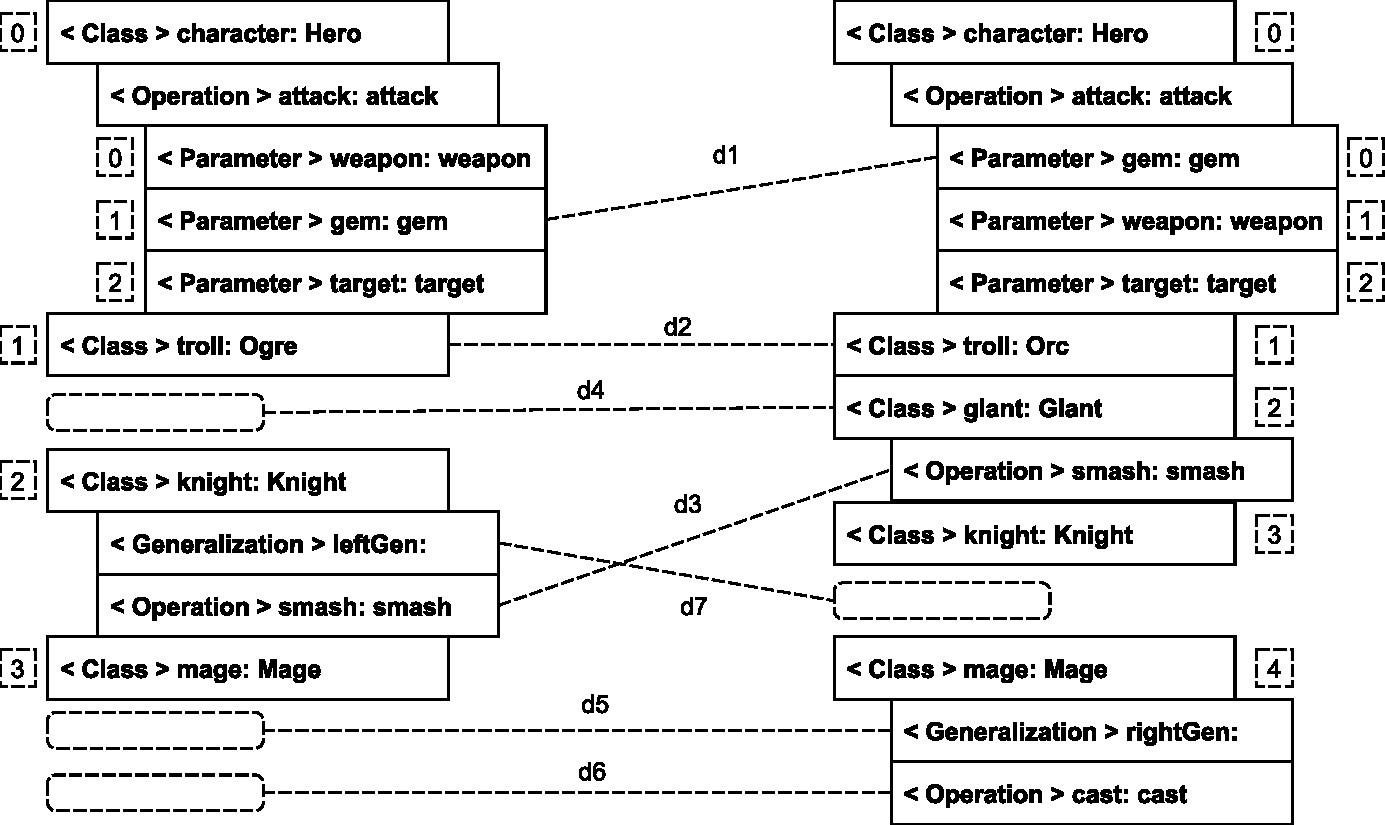
\includegraphics[width=\linewidth]{XmiComparison}
  \caption{A model comparison of the left and right models in Listings \ref{lst:xmimodel_left} and \ref{lst:xmimodel_right}.}
  \label{fig:xmi_comparison}
\end{figure}

\vspace{-20pt}
\begin{lstlisting}[firstnumber=1,style=eol,caption={The identified diffs presented as change events.},label=lst:readable_diffs]
move gem in attack.parameters from 0 to 1
set troll.name from "Orc" to "Ogre"
remove smash from giant.operations at 0 composite c1
add smash to knight.operations at 0 composite c1
unset giant.name from "Giant" to null composite c2
remove giant from resource at 2 composite c2
delete giant composite c2
unset mage.generalization from rightGen to null composite c3
unset rightGen.general from character to null  composite c3
delete rightGen composite c3
unset cast.name from "cast" to null composite c4
remove cast from mage.operations composite c4
delete cast composite c4
create leftGen type Generalization composite c5
set knight.generalization from null to leftGen composite c5
set leftGen.general from null to character composite c5
\end{lstlisting}

\section{State-based Conflict Detection}
\label{sec:emfcompare_conflict_detection}
In state-based model comparison, a conflict occurs when the states of an element or a feature are different in two different versions of a model that are being compared. In other words, it can be said that the applied change events that cause the difference are in conflict since they produce two different states -- in a previous shared version, these states are equal. State-based persistence does not record change events that cause the differences, thus the change events has to be derived through model differencing as in Section \ref{sec:state-based_model_differencing}. 

Let's say that we have three versions of a model, the original shared version $m_{o}$ and two other modified versions: the left version $m_{l}$ and the right version $m_{r}$. There are also two sets of derived operations, $C_{L}$ and $C_{R}$. These sets are obtained by differencing $m_{l}$ to $m_{o}$ and $m_{r}$ to $M_{O}$ using an LCS algorithm as explained in Section \ref{sec:state-based_model_differencing}, where $C_{L}$ = $\{c_{l1}$, $c_{l2}$, ..., $c_{olg}\}$, $C_{R}$ = $\{c_{r1}$, $c_{r2}$, ..., $c_{rh}\}$, $g = |C_{L}|$, and $h = |C_{R}|$. Applying $C_{L}$ to model $m_{o}$ transforms it into model $m_{l}$, and applying $C_{R}$ to model $m_{o}$ transforms it into model $m_{r}$. These derived change events are be used to detect conflicts using (\ref{eq:state_real_conflict}), (\ref{eq:state_pseudo_conflict}), and (\ref{eq:state_nonapplicability_conflict}).  

If the method in Section \ref{sec:state-based_model_differencing} is used -- as executed in EMF Compare -- to derive $C_{L}$ from the left and original versions -- Bob's and Jane's versions -- in Fig. \ref{fig:class_diagram_rpg} and present it in the format of change events, the following list are obtained. 
\begin{lstlisting}[firstnumber=1,style=eol,caption={The derived change events made by Bob to produce the right model in Fig. \ref{fig:class_diagram_left} (right version).},label=lst:cbp_left_state]
move target in attack.parameters from 1 to 2
set character.name from "Character" to "Hero"
set troll.name from "Troll" to "Ogre"
create leftGen type Generalization composite l1
set leftGen.general from null to character composite l1
set knight.generalization from null to leftGen composite l1
unset cast.name from "cast" to null composite l2
remove cast from giant.operations at 0 composite l2
delete cast composite l2
unset giant.name from "Giant" to null composite l3
remove giant from resource at 2 composite l3
delete giant composite l3
\end{lstlisting}

And following list is the derived change events for $C_{R}$ that are obtained from the right and original versions -- Alice's and Jane's versions -- in Fig. \ref{fig:class_diagram_rpg}. 
\begin{lstlisting}[firstnumber=1,style=eol,caption={The derived change events (operations) made by Alice to produce the right model in Fig. \ref{fig:class_diagram_right} (right version).},label=lst:cbp_right_state]
move gem in attack.parameters from 0 to 1
set character.name from "Character" to "Hero"
set troll.name from "Troll" to "Orc"
remove smash from knight.operations at 0 composite r1
add smash to giant.operations at 0 composite r1
create rightGen type Generalization composite r2
set rightGen.general to character composite r2
set mage.generalization to rightGen composite r2
remove cast from giant.operations at composite r3
add cast to mage.operations at 0 composite r3
\end{lstlisting}

\textbf{Real Conflict}. In state-based model comparison, two change events, $c_{l}$ and $c_{r}$, are in conflict if both are applied to a same element $e_{o}$ but produce two different eventual states where $!$ is used as the operator for expressing that two change events are in conflict (\ref{eq:state_real_conflict}). EMF Compare \cite{emfcompare2018developer} classifies this conflict as a \textsf{REAL} conflict. For example, Bob changed the \textsf{name} of \textsf{troll} to ``Ogre'' (Listing \ref{lst:cbp_left_state}) while Alice modified it to ``Orc'' (Listing \ref{lst:cbp_right_state}). 
\begin{equation} \label{eq:state_real_conflict}
e_{o} + c_{l} \not\equiv e_{o} + c_{r} \Rightarrow c_{l}\;!\;c_{r}
\end{equation} 
\textbf{Non-applicability}. A \textsf{REAL} conflict also occurs when applying a change event $c_{l}$ to element $e_{o}$ makes $c_{r}$ inapplicable to element $e_{o}$. Therefore, change events $c_{l}$ and $c_{r}$ are in conflict (\ref{eq:state_nonapplicability_conflict}). 
For instance, Alice moved operation \textsf{smash} from class \textsf{Knight} to class \textsf{Giant} (Listing \ref{lst:cbp_right_state}) but this class was deleted by Bob (Listing \ref{lst:cbp_left_state}). Deleting class \textsf{Giant} makes the move inapplicable. 
\begin{equation} \label{eq:state_nonapplicability_conflict}
(e_{o} + c_{r} \not\equiv e_{o}) \wedge (e_{o} + c_{l} + c_{r} \equiv e_{o} + c_{l}) \Rightarrow c_{l}\;!\;c_{r}
\end{equation}
\textbf{Pseudo Conflict}. A conflict is classified as \textsf{PSEUDO} if the eventual states produced are equivalent. The \textsf{PSEUDO} means the conflict can be automatically resolved by choosing any of the conflicting changes since any of the changes produces the same eventual states (\ref{eq:state_pseudo_conflict}). Symbol $!_{p}$ is used as the operator for expressing that two change events are in \textsf{PSEUDO} conflict. For example, both Bob and Alice changed the \textsf{name} of element \textsf{character} from ``Character'' to ``Hero'' (Listings \ref{lst:cbp_left_state} and \ref{lst:cbp_right_state}). 
\begin{equation} \label{eq:state_pseudo_conflict}
e_{o} + c_{l} \equiv e_{o} + c_{r} \Rightarrow c_{l}\;!_{p}\;c_{r}
\end{equation} 

\begin{table}[h]
  \centering
  \caption{Conflicting change events identified using EMF Compare based on the case in Fig. \ref{fig:class_diagram_rpg}.}
  \label{table:emfc_conflicts}
  % Please add the following required packages to your document preamble:
  % \usepackage[table,xcdraw]{xcolor}
  % If you use beamer only pass "xcolor=table" option, i.e. \documentclass[xcolor=table]{beamer}
  
  \begin{scriptsize}
  \begin{tabular}{|l|p{5cm}|p{5cm}|l|}
    \hline
    \multicolumn{1}{|c|}{{\textbf{ID}}} & 
    \multicolumn{1}{p{5cm}|}{{\textbf{Left Change Events (Bob)}}} & \multicolumn{1}{p{5cm}|}{{\textbf{Right Change Events (Alice)}}} & \multicolumn{1}{c|}{{\textbf{Type}}}\\ 
    \hline
    EC1                                                      & set character.name from "Character" to "Hero"                                 & set character.name from "Character" to "Hero"                                                                         & \begin{tabular}[c]{@{}l@{}}pseudo\\conflict\end{tabular} \\ \hline
    EC2                                                      & set troll.name from "Troll" to "Ogre"                                         & set troll.name from "Troll" to "Orc"                                                                                  & \begin{tabular}[c]{@{}l@{}}real conflict\end{tabular}        \\ \hline
    EC3                                                      & delete cast                                                                  & \begin{tabular}[c]{@{}l@{}}remove cast from giant.operations at 1\\ add cast to mage.operations at 0\end{tabular}     & \begin{tabular}[c]{@{}l@{}}non-\\ applicability\end{tabular}        \\ \hline
    EC4                                                      & delete giant                                                                   & \begin{tabular}[c]{@{}l@{}}remove smash from knight.operations\\ 
      \,\, at 0\\ 
      add smash to giant.operations at 0
    \end{tabular} & 
    \begin{tabular}[c]{@{}l@{}}non-\\ applicability\end{tabular}        \\ \hline
  \end{tabular}
  \end{scriptsize}
\end{table}

Using (\ref{eq:state_real_conflict}), (\ref{eq:state_nonapplicability_conflict}), and (\ref{eq:state_pseudo_conflict}) and information in Listings \ref{lst:cbp_left_state} and \ref{lst:cbp_right_state}, four conflicts can be identified -- presented in Table \ref{table:emfc_conflicts} along with their conflicting change events. Conflict \textsf{EC1} is a \textsf{pseudo} conflict since both modify the same class \textsf{character}'s feature \textsf{name} resulting the same end states, ``Hero'' or ``Hero''. Conflict \textsf{EC2} is a \textsf{REAL} conflict. Applying changing \textsf{troll}'s \textsf{name} to ``Ogre'' and \textsf{troll}'s \textsf{name} to ``Orc'' produces two different states -- ``Ogre'' and ``Orc''. Conflicts \textsf{EC3} and \textsf{EC4} are \textsf{REAL} non-applicability conflicts since if operation \textsf{cast} is deleted first then it cannot be moved -- removed and added -- from class \textsf{giant}'s \textsf{operations} to class \textsf{mage}'s \textsf{operations}, and if class \textsf{giant} is deleted first then operation \textsf{smash} cannot be moved -- removed and added -- from  class \textsf{knight}'s \textsf{operations} to class \textsf{giant}'s \textsf{operations}.

Conflict detection in state-based comparison might not be accurate since the derived differences/change events might not reflect the real historical changes of a model. For example, EMF Compare \cite{emfcompare2018developer}, a tool that perform state-based model comparison, does not detect that Alice and Bob modified the same element -- parameter \textsf{target} -- as indicated by line 29 in List. \ref{lst:cbp_right} and line 35 in List. \ref{lst:cbp_left}. Using an LCS algorithm, the derived change events related to the feature \textsf{parameters} of element \textsf{attack}, which if presented as change events, are expressed as [\textsf{\small \textbf{move} target \textbf{in} attack.parameters \textbf{from} 1 \textbf{to} 2}] for Bob's version and [\textsf{\small \textbf{move} gem \textbf{in} attack.parameters \textbf{from} 1 \textbf{to} 2}] for Alice's version. Using (\ref{eq:conflict_1.3}), both change events are not in conflict since both change events modify two different elements, \textsf{target} and \textsf{gem}. The result is different if change-based approach is employed to detect conflicts using the change event records in Listings \ref{lst:cbp_left} and \ref{lst:cbp_right} which is explained in Section \ref{sec:emfstore_conflict_detection}.

\section{Change-based Conflict Detection}
\label{sec:emfstore_conflict_detection}
EMF Store \cite{koegel2010emfstore} is a product that implements change-based model persistence for EMF models. It is a collaborative repository and versioning system that is specifically designed for models to answer existing versioning systems, such as Git and SVN, that focus heavily on text-based files \cite{emfstore2019what}. EMF Store follows the following rules to identify conflict between change events \cite{koegel2010operation}. 

\textbf{Non-commutability}. In EMF Store, change events $c_{l}$ and $c_{r}$ are in conflict if applying them in different order to a same element $e_{o}$ produces two different eventual states. For example, Alice changed the \textsf{name} of class \textsf{Troll} to ``Orc'' (Listing \ref{lst:cbp_right}) while Bob renamed it to ``Ogre'' (Listing \ref{lst:cbp_left}). Applying Alice's change first to Bob's change results in the class' \textsf{name} equals to ``Ogre'', or ``Orc'' if the order is reversed.
\begin{equation} \label{eq:change_noncommutability}
e_{o} + c_{l} + c_{r} \not\equiv e_{o} + c_{l} + c_{r} \Rightarrow c_{l}\;!\;c_{r}
\end{equation}  
However, after examining the implementation \cite{eclipse2019emfstore}, even though two different change events produce equivalent eventual states, both change events are still treated in conflict by EMF Store. For example, both Bob and Alice changed the \textsf{name} of element \textsf{character} from ``Character'' to ``Hero'' (Listing \ref{lst:cbp_left} line \ref{line:cbp_left_34} and Listing \ref{lst:cbp_right} line \ref{line:cbp_right_39}). The reason is if we apply Bob's set event first, it changes \textsf{character}'s \textsf{name} from ``Character'' to ``Hero''. It is important to notice that after applying Bob's set event, the eventual value of \textsf{character}'s \textsf{name} is ``Hero''. Applying Alice's set event with previous value ``Character'' is inapplicable since it makes the sequence of the change events inconsistent; Bob's set event produces end value ``Hero'' which is not the previous value changed by Alice's set event, which is ``Character''. The same inconsistency still occurs even we apply these set events in different order.

\textbf{Co-modifiability}. Thus, this leads to a new definition that conflict occurs when two different change events modify a same element or feature regardless the equivalency of the eventual states that they produce. 
\begin{equation} \label{eq:change_comodifiabilty}
(e_{o} + c_{l} \equiv e_{o} + c_{r}) \vee (e_{o} + c_{l} \not\equiv e_{o} + c_{r}) \Rightarrow c_{l}\;!\;c_{r}
\end{equation} 
\textbf{Non-applicability}. This non-applicability rule is the same with the non-applicability rule in the state-based conflict detection. Essentially, a conflict occurs when applying a change event $c_{l}$ to element $e_{o}$ makes $c_{r}$ inapplicable to element $e_{o}$. For instance, Alice moved operation \textsf{smash} from class \textsf{Knight} to class \textsf{Giant} (Listing \ref{lst:cbp_right}) but this class was deleted by Bob (Listing \ref{lst:cbp_left}). Deleting class \textsf{Giant} makes the move inapplicable. 
\begin{equation} \label{eq:change_nonapplicability}
(e_{o} + c_{r} \not\equiv e_{o}) \wedge (e_{o} + c_{l} + c_{r} \equiv e_{o} + c_{l}) \Rightarrow c_{l}\;!\;_{r}
\end{equation}
\textbf{Composite}. If change event $c_{l}$ is in conflict with change event $c_{r}$ where $c_{r}$ is a member of a set of composite change event $cc_{r}$ then change event $c_{l}$ is also in conflict with each change event $c_{n}$ in composite change event $cc_{r}$. For example, the deletion of class \textsf{Giant} is part of composite event \textsf{l2} (Listing \ref{lst:cbp_left}) and the addition of operation \textsf{smash} to class \textsf{Giant} is part of composite event \textsf{r1} (Listing \ref{lst:cbp_right}). Since they are in conflict according to (\ref{eq:change_nonapplicability}), all other change events in their composite events, \textsf{l2} and \textsf{r1}, are also in conflict.
\begin{equation} \label{eq:change_composite}
c_{l}\;!\;c_{r} \wedge c_{r} \in cc_{r} \Rightarrow c_{l}\;!\; \forall c_{rn} | c_{rn} \in cc_{r}
\end{equation}

\begin{table}[ht]
  \centering
  \caption{Conflicting change events identified using EMF Store in Listings \ref{lst:cbp_right} and \ref{lst:cbp_left}.}
  \label{table:conflicts_emfs}
  \begin{scriptsize}
  \begin{tabular}{|l|p{5cm}|p{5cm}|l|}
    \hline
    \multicolumn{1}{|c|}{\textbf{ID}} & 
    \multicolumn{1}{c|}{\textbf{Left Change Events (Bob)}} & 
    \multicolumn{1}{c|}{\textbf{Right Change Events (Alice)}} & 
    \multicolumn{1}{c|}{ \textbf{Type}} \\ 
    \hline
    \multirow{2}{*}{ES1} & set troll.generalization from null to leftGen                                                                                                                                                                              & \begin{tabular}[c]{@{}l@{}}unset troll.generalization from rightGen\\
      \,\,to null\\set mage.generalization from null to\\ \,\,rightGen\end{tabular} & \multirow{2}{*}{\begin{tabular}[c]{@{}l@{}}co-\\modifiability\\ composite\end{tabular}}                                                                                             \\ \cline{2-3}
    & \begin{tabular}[c]{@{}l@{}}unset troll.generalization from leftGen\\
      \,\, to null\\ set knight.generalization from null\\
      \,\, to leftGen\end{tabular}                       
    & set troll.generalization from null to rightGen                                                                                             &  \\ \hline
    ES2                                                      & set character.name from "Character" to"Hero"                                                                                                                                                                               & set character.name from "Character" to "Hero"                                                                                             & \begin{tabular}[c]{@{}l@{}}co-\\modifiability\end{tabular}                          \\ \hline
    ES3                                                      & move target in attack.parameters from 1 to 2                                                                                                                                                                               & move target in attack.parameters from 1 to 0                                                                                              & \begin{tabular}[c]{@{}l@{}}non-\\ applicability\end{tabular}                                 \\ \hline
    \multirow{2}{*}{ES4} & \multirow{2}{*}{\begin{tabular}[c]{@{}l@{}}unset cast.name from "cast" to null\\ remove cast from giant.operations\\
        \,\,at 0\\ delete cast type Operation\\ unset giant.name from "Giant" to null\\ delete giant\end{tabular}}                                                         & \begin{tabular}[c]{@{}l@{}}remove cast from giant.operations at 0\\ add cast to mage.operations at 0 \end{tabular}                         
    & \multirow{2}{*}{\begin{tabular}[c]{@{}l@{}}non-\\applicability\\ composite\end{tabular}} \\ \cline{3-3}
    &  & \begin{tabular}[c]{@{}l@{}}remove smash from knight.operations\\
      \,\,at 0\\ add smash to giant.operations at 1\\ \\ \\ \end{tabular}                     &   \\ \hline
    
    ES5                                                      & set troll.name from "Troll" to "Ogre"                                                                                                                                                                                      & set troll.name from "Troll" to "Orc"                                                                                                      & \begin{tabular}[c]{@{}l@{}}co-\\modifiability\end{tabular}                                 \\ \hline
  \end{tabular}
\end{scriptsize}
\end{table}

In change-based conflict detection, all change events applied to a model are already available in change-based persistence, thus the change events do not need to be derived trough a diffing process. The availability of real historical changes can improve the accuracy of change detection since elements that have been changed can be identified according to fact -- not derivation. In consequence, it can detect conflicts that cannot be detected by state-based conflict detection. For example, in Listing \ref{lst:cbp_right} line 31, parameter \textsf{target} has been moved from index 1 to 0, while in Listing \ref{lst:cbp_left} line 37, it was moved from index 1 to 2. Since both change events modified the same parameter \textsf{target}, both change events can be identified in conflict using (\ref{eq:change_comodifiabilty}); the same parameter \textsf{target} is modified by two different change events. 


The drawback of EMF Store is that it treats two change events that modify a same element as they are in conflict regardless of the end states that they produce to the element \cite{DBLP:conf/sfm/BroschKLSWW12}. In common sense, two changes should not be in conflict if they are applied to a same element or feature and produce same eventual states. Moreover, EMF Store it does not have a classification that separates conflicts into \textsf{REAL} or \textsf{PSEUDO} conflicts, such as in EMF Compare, to automate conflict resolution. For example, two change events in Listing \ref{lst:cbp_right} at line \ref{line:cbp_right_39} and Listing \ref{lst:cbp_left} at line \ref{line:cbp_left_35}, that change the same feature \textsf{name} from ``Character'' to the same value ``Hero'', are treated in conflict (Table \ref{table:conflicts_emfs} id ES2) using (\ref{eq:change_comodifiabilty}). EMF Compare classifies this kind of conflict as \textsf{PSEUDO} conflict which can be automatically resolved in merging only by selecting one of the conflicting change events and ignoring the other one.

Excluding eventual states in detecting conflicts also causes all change events related to \textsf{troll}'s \textsf{generalization} to be in conflict; all the feature's left-side events are in conflict with all its right-side events (Table \ref{table:conflicts_emfs}, ES1). Using the co-modifiability  (\ref{eq:change_comodifiabilty}) rule, we can detect that the setting and unsetting of \textsf{troll}' \textsf{generalization} to \textsf{leftGen} and \textsf{null} (Listing \ref{lst:cbp_left} lines \ref{line:cbp_left_33}, \ref{line:cbp_left_35}) are in conflict with the setting and unsetting of \textsf{troll}' \textsf{generalization} to \textsf{rightGen} and \textsf{null} (Listing \ref{lst:cbp_right} lines \ref{line:cbp_right_38}, \ref{line:cbp_right_40}). Moreoever, using composite (\ref{eq:change_composite}) rule, we can also identify that the setting of \textsf{knight}' \textsf{generalization} to \textsf{leftGen} (Listing \ref{lst:cbp_left} line \ref{line:cbp_left_36}) and the setting of \textsf{mage}' \textsf{generalization} to \textsf{rightGen} (Listing \ref{lst:cbp_right} line \ref{line:cbp_right_41}) are also part of the conflict ES1 since both events are in the same composite move events, \textsf{l1} and \textsf{r3}, with the unsetting of \textsf{troll}' \textsf{generalization} to  \textsf{null} (Listing \ref{lst:cbp_left} line \ref{line:cbp_left_35}, Listing \ref{lst:cbp_right} line \ref{line:cbp_right_38}).

In state-based conflict detection, case ES1 is not a conflict since the values of class \textsf{troll}'s feature \textsf{generalization} in the Jane's, Bob's, and Alice's versions are indentical -- all are null. Thus, there are no different \textit{derived} change events that modify class \textsf{troll}'s feature \textsf{generalization} in parallel. 

Conflict ES4 is a non-applicability, composite conflict. Moving element \textsf{smash} from class \textsf{knight} to class \textsf{giant} and moving element \textsf{cast} from class \textsf{giant} to class \textsf{mage} require the deletion of class \textsf{giant} to be executed later in order to be applicable. Conflict ES5 is can be detected with the co-modifiability  (\ref{eq:change_comodifiabilty}) rule. The states of \textsf{troll}'s \text{name} have been simultaneously modified to ``Ogre'' or ``Orc''.

The summary of the advantages and drawbacks between EMF Compare and EMF Store in detecting conflicts are presented in Table \ref{tab:accuracy_emfcompare_emfstore}.

\begin{table}[ht]
  \centering
  \caption{The advantages and drawbacks of EMF Compare and EMF Store in detecting conflicts.}
  \label{tab:accuracy_emfcompare_emfstore}
\begin{tabular}{|p{0.14\linewidth}|p{0.38\linewidth}|p{0.38\linewidth}|}
    \hline
    & \textbf{State-based Conflict Detection (EMF Compare)}
    & \textbf{Change-based Conflict Detection (EMF Store)}\\
    \hline
    \multicolumn{1}{|c|}{Advantages}
    &
    \begin{minipage}[t]{\linewidth}
    \raggedright
    \begin{itemize}[leftmargin=9pt]
      \setlength\itemsep{2pt}
      \item[-] detect \textsf{PSEUDO} conflict which can be automatically resolved when merging
      \item[-] conflicts detected are optimal since changes are derived thus avoid oversensitive conflict detection
      \item[]
    \end{itemize}
    \end{minipage}
    &
    \begin{minipage}[t]{\linewidth}
      \raggedright
    \begin{itemize}[leftmargin=9pt]
      \setlength\itemsep{2pt}
      \item[-] more accurate in detecting conflicts since changes are real history
      \item[]
    \end{itemize} 
  \end{minipage}
    \\ 
    \hline
    \multicolumn{1}{|c|}{Drawbacks}
    &
    \begin{minipage}[t]{\linewidth}
      \raggedright
    \begin{itemize}[leftmargin=9pt]
      \setlength\itemsep{2pt}
      \item[-] less accurate in detecting conflicts since changes are derived -- not real changes
      \item[-] in large models, its performance should be slower the change-based approach since it performs 3-way comparison which requires 2-times model differencing to derive changes 
      \item[]
    \end{itemize}
    \end{minipage}
    &
    \begin{minipage}[t]{\linewidth}
      \raggedright
    \begin{itemize}[leftmargin=9pt]
      \setlength\itemsep{2pt}
      \item[-] treat all conflicts as \textsf{REAL} conflicts which demand user intervention for resolution
      \item[-] can be oversensitive in detecting conflicts since eventual states are not considered
      \item[-] in large models with moderate changes, it should perform faster than the state-based approach -- no need to derive changes since they are available already 
      \item[]
    \end{itemize} 
  \end{minipage}
    \\
    \hline                         
  \end{tabular}
\end{table}

\section{Research Method}
\label{sec:research_method}
In performing this research, this work follows the experiment process proposed by Wohlin et al. \cite{DBLP:books/daglib/0029933/Wohlin}. The experiment process consist of 5 activities: scoping, planning, operation, analysis and interpretation, and presentation and package.

\textbf{Scoping}. In the scoping activity, the hypothesis, goals, and objectives of an experiment have to be defined clearly \cite{DBLP:books/daglib/0029933/Wohlin}. Basili et al. \cite{basili1988tame} provide the following questions (scoping points) in their framework to help determining the scope of an experiment in software engineering: (1) what is studied? (object of study), (2) what is the intention? (purpose), (3) which effect is studied? (quality focus), (4) whose view? (perspective), and where is the study conducted? (context).

%This work studies change-based model persistence as an alternative method for persisting models. The study includes defining methods to load and save change-based models as well as to reduce the main drawback of the persistence -- the slow loading of change-based models. This work also investigates a method in leveraging the persistence to produce a faster model differencing and conflict detection. It is expected that change-based model persistence can support modellers/developers to improve the efficiency of their model management in the context of model-driven engineering.

\textbf{Planning}. In the planning activity, these components have to be defined in detail: context selection, hypothesis formulation, variables selection, selection of subjects, experiment design selection, instrumentation, and validity evaluation\cite{DBLP:books/daglib/0029933/Wohlin}. The context can be offline vs. online, student vs. professional, toy vs. real problems, specific vs. general. Null and alternative hypotheses have to be stated formally and the data gathered throughout the experiment should be used, using appropriate statistical tests, to reject the null hypothesis if possible. In the variables selection, we determine the independent and dependent variables to be measured. The subjects should be selected carefully that they are representative to the case experimented in order to generalise the results of the experiment. To get the desired results, experiment should be designed carefully and suitable standard design types should be selected. Experiment objects, guidelines, and measurement instruments also should be defined to ensure the experiment is executable. Lastly the validity threats should be identified and evaluated.

\textbf{Operation}. The operation activity consists of three steps: preparation, execution, and validation \cite{DBLP:books/daglib/0029933/Wohlin}. 
In the preparation, we select and inform participants and prepare all the required materials to facilitate the execution of the experiment. The experiment can be executed in a number of ways, such as in one or multiple occasions, or in one or multiyear.  While the executing, we have to make sure that the experiment is on the right track, not interrupted, and running correctly. We also have to validate the produced data if they are reasonable and collected correctly. 

\textbf{Analysis and interpretation}.
To understand the data gathered, descriptive statistics and visualization can be used. We can also remove unnecessary data and variables to facilitate analysis and interpretation. We can then perform hypothesis testing to reject or accept the experiment's hypotheses. The analysis and interpretation should explain how the data gathered contribute to the rejection or acceptance of the hypotheses. The results might be statistically insignificant, but the lessons might still worth to be learned \cite{DBLP:books/daglib/0029933/Wohlin}. 

\textbf{Presentation and package}. In this activity, experiment results should be documented and published in research papers for the dissemination of the results. The experiment also should be packaged to support other parties to replicate it \cite{DBLP:books/daglib/0029933/Wohlin}. 
